\documentclass[11pt, a4paper]{article}
\usepackage{sectsty}
\usepackage{graphicx}
\usepackage{amsmath}
\usepackage{amssymb}
\usepackage{setspace}
\usepackage{tasks}
\usepackage{graphicx}
\usepackage{float}
\usepackage{comment}
\usepackage{listings}
\usepackage[utf8]{inputenc}
\usepackage{amsfonts}
\usepackage{gensymb}
\usepackage{multicol}
\usepackage{tabularx}
\usepackage{tikz}
\newcommand{\myvec}[1]{\ensuremath{\begin{pmatrix}#1\end{pmatrix}}}
\let\vec\mathbf

\newcommand{\mydet}[1]{\ensuremath{\begin{vmatrix}#1\end{vmatrix}}}
\providecommand{\brak}[1]{\ensuremath{\left(#1\right)}}
\providecommand{\lbrak}[1]{\ensuremath{\left(#1\right.}}
\providecommand{\rbrak}[1]{\ensuremath{\left.#1\right)}}
\providecommand{\cbrak}[1]{\ensuremath{\left\{#1\right\}}}
\providecommand{\sbrak}[1]{\ensuremath{{}\left[#1\right]}}
\providecommand{\norm}[1]{\left\lVert#1\right\rVert}
\providecommand{\abs}[1]{\left\vert#1\right\vert}

\title{ Math computing}
\author{ Yaswanth }
\date{\today}

\begin{document}
\vspace{-\baselineskip}
\maketitle

\section*{NCERT 9.7.1.5}

\textbf{This question is from class 9 ncert chapter 7.triangles}
\begin{enumerate}
    \item Line $l$ is the bisector of an angle $\angle A$ and $B$ is any point on $l$. $BP$ and $BQ$ are perpendiculars from $B$ to the arms of $\angle A$. Show that:
%
\begin{enumerate}
    \item $\triangle  APB \cong \triangle AQB$  
    \item $BP$ = $BQ$ or $B$ is equidistant from the arms of $\angle A$.
 \end{enumerate}
\end{enumerate}
\begin{figure}[H]
    \centering
    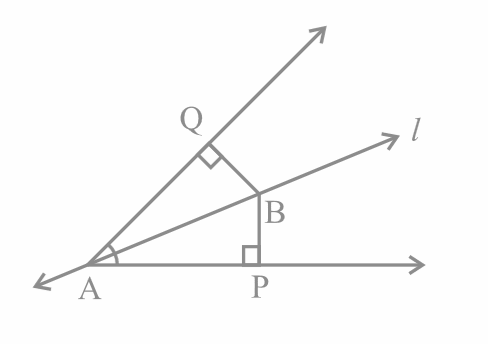
\includegraphics[width=1\columnwidth]{fig_mc.png}
    \caption{$\triangle AQB \hspace{12pt} and \hspace{12pt} \triangle APB$}
    \label{fig:math_comp1}
\end{figure}
\pagebreak
\textbf{Construction steps:}
%
\begin{enumerate}
\item
\begin{enumerate}

\item let ,consider the point $A$ be the origin 
\begin{align}
\vec{A} &= \myvec{0 \\ 0}
\end{align}

\item Assuming the distance between point $A$ and $B$ be $5$ ,and also considering the point $B$ on same axis ,So
\begin{align}
\vec{B} &= \myvec{5 \\ 0}
\end{align}

\item let assume the distance between point $A$ and $P$ be $4$ ,and let the line $AB$ makes an angle $30 \degree$ anticlock wise with line $AP$.
\begin{align}
r &= 4  \\
\angle PAB &= \theta = 30 \degree
\end{align}

\item Now the coordinates of point $P$ will be,
\begin{align}
\vec{P} &= \myvec{r \cos \theta \\ -r \sin \theta} \\
	&= \myvec{4 \cos 30 \degree \\ -4 \sin 30 \degree} \\
\text{on calculating} \nonumber \\
\vec{P} &= \myvec{3.464101 \\ -2} 
\end{align}

\item Similarly , let assume the distance between point $A$ and $Q$ also be $4$ , and the line $AB$ makes an angle $30 \degree$ clock wise with line $AQ$. Now the coordinates of point $Q$ be,
\begin{align}
\angle QAB &= \theta = 30 \degree \\
\vec{Q} &= \myvec{r \cos \theta \\ r \sin \theta} \\
	&= \myvec{4 \cos 30 \degree \\ 4 \sin 30 \degree} \\
\text{on calculating} \nonumber \\
\vec{Q} &= \myvec{3.464101 \\ 2} 
\end{align}

\item Now the coordinates of $A$,$B$,$P$,$Q$ are calculated .
\begin{align}
\vec{A} &= \myvec{0 \\ 0},\,
\vec{B} &= \myvec{5 \\ 0} ,\,
\vec{P} &= \myvec{3.464101 \\ -2} ,\,
\vec{Q} &= \myvec{3.464101 \\ 2} 
\end{align}
Joining these points forms the required figure

\end{enumerate}

\end{enumerate}

\begin{figure}[H]
    \centering
    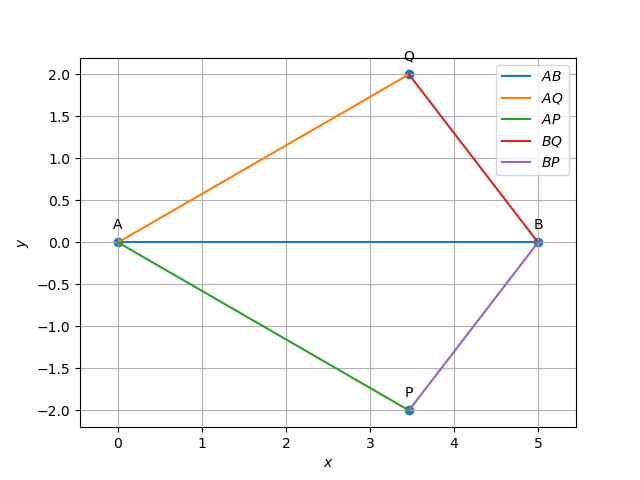
\includegraphics[width=\columnwidth]{fig_mat_comp.png}
    \caption{$\triangle APB \hspace{12pt} and \hspace{12pt} \triangle AQB$}
    \label{fig:math_comp2}
\end{figure}


\end{document}
